%%%%%%%%%%%%%%%%%%%%%%%%%%%%%%%%%%%%%%%%%%%%%%%%%%%%%%%%%%%
% PAPER ON AGGRESSION AND MISOGYNY DETECTION
% HOSTED WITH - SANDIP DUTTA
%%%%%%%%%%%%%%%%%%%%%%%%%%%%%%%%%%%%%%%%%%%%%%%%%%%%%%%%%%%
\documentclass[conference]{IEEEtran}
%---------PREAMBLE------------
% \IEEEoverridecommandlockouts
% The preceding line is only needed to identify funding in 
% the first footnote. If that is unneeded, please comment it out.
% ---------PACKAGES DECLARED HERE---------
\usepackage{cite}
\usepackage{amsmath,amssymb,amsfonts}
\usepackage{algorithm}
\usepackage{algorithmic}
\usepackage{graphicx}
\usepackage{textcomp}
\usepackage{xcolor}
% -------Hyperref-Generating Hyperlinks------------
\usepackage{hyperref}
\hypersetup{colorlinks=true,linkcolor=blue,pdftitle={An Efficient BERT Aided Pipeline to Detect Aggression and Misogyny},pdfpagemode=FullScreen,}
\usepackage{tabularx}
% ------------------------
\def\BibTeX{{\rm B\kern-.05em{\sc i\kern-.025em b}\kern-.08em
    T\kern-.1667em\lower.7ex\hbox{E}\kern-.125emX}}
% ----DOCUMENT-----------------------------
\begin{document}
%-----------TITLE---------------
\title{An Efficient BERT Aided Pipeline to Detect Aggression and Misogyny}
%------------AUTHORS-----------------------
\author{
\IEEEauthorblockN{1\textsuperscript{st} Given Name Surname}
\IEEEauthorblockA{\textit{dept. name of organization (of Aff.)} \\
\textit{name of organization (of Aff.)}\\
City, Country \\
email address or ORCID}
\and
\IEEEauthorblockN{2\textsuperscript{nd} Given Name Surname}
\IEEEauthorblockA{\textit{dept. name of organization (of Aff.)} \\
\textit{name of organization (of Aff.)}\\
City, Country \\
email address or ORCID}
\and
\IEEEauthorblockN{3\textsuperscript{rd} Given Name Surname}
\IEEEauthorblockA{\textit{dept. name of organization (of Aff.)} \\
\textit{name of organization (of Aff.)}\\
City, Country \\
email address or ORCID}
}
%-----------MAIN------------
%-----------TITLE-----------
\maketitle
%-----------ABSTRACT--------
\begin{abstract}
    Social media is bustling with ever growing cases of trolling, aggression and hate. A huge amount of data is generated each day which is insurmountable for manual inspection. In this work, we propose an efficient and fast pipeline to detect aggression and misogyny in social media texts. We use data from the Second Workshop on Trolling, Aggression and Cyber Bullying for our task. We employ a BERT based pipeline to augment our data. Next we employ Tf-Idf and XGBoost based pipeline for detecting aggression and misogyny. Our model achieves 0.73 and 0.85 (both Weighted F1 Score) on the 2 prediction tasks, which ranks very close to the state of the art. However, the training time, model size and resource requirements are drastically reduced compared to state of the art models, making our proposed pipeline useful for fast inference. We describe the pipeline, examine the results and conduct error analysis to understand the shortcomings of our model.
\end{abstract}
%----------KEYWORDS---------
\begin{IEEEkeywords}
Cyberbully Detection, Aggression Detection, Sentiment Analysis, BERT, Data Augmentation
\end{IEEEkeywords}
%----------INTRODUCTION-----
\section{Introduction}
Social media has been an important platform for people to voice their opinions. 
However, with the rise of social media, there has also been a huge surge of online criticism and trolling. 
Due to the constant stream of information and the need to achieve perfectionism due to the fear of trolling, physical as well as mental health is deteriorating. 
Mitigation of these kinds of online bullying has been an important problem and has been studied for a long time. 

However, the amount of information generated on social media is too large for humans to wade through. As part of the effort to better organize this information and detect online trolling, researchers have been actively investigating the problem of automatic text categorization. Rule based models and statistical techniques have been developed that can understand the properties of text data and can predict whether there is any trolling present in the data or not.

Machine Learning (ML) models have achieved great success in this task of text categorization. With the advent of deep learning and availability of high end computational resources, the performance has increased manifold. With newer and larger models being built, the ability of deep learning to solve complicated tasks with very high accuracy is evident. 

But even as larger models with better and better accuracy are being built, the importance of the quality of data has still not reduced. Larger models will give sub optimal results if the data they are trained on is not of good quality. But the results of large models are more difficult to interpret. Traditional ML models also have the advantage of giving results that are relatively easier to interpret.
With these ideas in mind, we have developed our text classification pipeline.

In this work, we use a large deep learning model and traditional ML approaches for the purpose of text classification. The data contains social media texts from YouTube comments. We have to predict the presence of aggression and misogyny from the given data. We first explore the data set to reveal some class distribution issues with the data. Next we develop a Bidirectional Encoder Representations from Transformers(BERT)\cite{devlin2019bert} based text data augmentation pipeline to fix the data distribution. This augmented data helps to reduce class imbalance. For the classification pipeline, we develop a Tf-Idf and XGBoost based classification pipeline to classify the text. 

Our model
\footnote{Source Code : \url{https://github.com/Dutta-SD/AggDetect}}
achieves a score very close to the state of the art. However, as the augmentation task is essentially a one time process, our model is simpler and faster. The main classification pipeline does not require us to use high end computational resources during inference, which makes our model even more convenient to use.

%-----RELATED WORK---------------------

\section{Related Works}

Recent work in the domain of identifying text-based aggression, cyberbullying and hate speech on social media and other online spheres, has advanced in the past few years. This area of study has gathered the focus of researchers interested in linguistic features of aggression, and from computer scientists interested in developing tools to detect and process aggressive content on social media platforms. In this section, we cite some of the studies and briefly discuss their findings. 

So far, significant contributions have been made in the domain of aggression detection in text, in the field of natural language processing, through the likes of \cite{razavi2010offensive} \cite{kumar2018trac}\cite{kumar2020evaluating}. 
Other aspects of similar text detection has been found in areas of trolling \cite{cambria2010not}\cite{mihaylov2015finding}\cite{de2018modeling}, 
misogyny \cite{anzovino2018automatic}, 
cyberbullying \cite{dadvar2013improving}\cite{xu2012learning}, 
racism \cite{greevy2004automatic}, 
offensive language\cite{nobata2016abusive}, 
hate speech\cite{inproceedings}\cite{davidson2017automated}. 
All these works are diverse in terms of the target subject they investigate. The works have mainly been conducted on the English language data sets, but there are various languages on which the experiments have been recorded, for example, in Hindi\cite{mandla2021overview}, in Spanish\cite{garibo-i-orts-2019-multilingual}, in Chinese\cite{su-etal-2017-rephrasing}, etc.

\subsection{BERT-based Work}
BERT is a pre-trained text encoder, that rapidly advances the state of the art on many NLP tasks. Some relevant works that have explored BERT, are \cite{tenney2019bert} on the groundbreaking potential of BERT pipelines in classical NLP, \cite{wan2021enhancing} studies its effectiveness when the target domain is shifted from the pre-training corpora, \cite{sachidananda2021efficient} an alternative approach by adapting their tokenizers to provide strong performance, \cite{azhar2021finetuning} an aspect-based sentiment analysis using BERT pipelines, etc.

\subsection{Text Data Cleaning}
Before the process of vectorization, we need to perform a sequence of operations on the text, so that our text can be “cleaned” out. Some important works that employ this are \cite{rahm2000data} which enlists the domain of data cleaning, \cite{esuli2009training} which addresses the strategies necessary for effective cleaning performances in supervised structures, \cite{tang2005email} which deals with email data cleaning for text mining, etc.

\subsection{Tf-Idf Vectorizer}
Tf-Idf is the most frequently used algorithm to convert the text into vectors.
\cite{kalra2019automatic} makes use of the Tf-Idf features to classify pathology reports. 
\cite{dutta2021sequencetosequence} proposes a novel learning framework which uses Tf-Idf based keyword extraction, to assist their experiment of efficient FAQ retrieval. \cite{lepekhin2021experiments} explores adversarial attacks on text genres, by employing Tf-Idf for keyword extraction. 
Some other prominent works include
\cite{fattahi2020spaml}, 
\cite{ma2020xtqa}, etc.

\subsection{XGBoost Classifier}
XGBoost works as Newton-Raphson in function space unlike gradient boosting that works as gradient descent in function space. In the work of Aspect-based Sentiment Analysis \cite{azhar2021finetuning}, XGBoost method has been used to generalize well in test data and better classification.
\cite{kalra2019automatic} employs the XGBoost to classify pathology reports.
\cite{septiandri2017predicting} explores the method in classifying Indonesian names on the basis of gender.
\cite{jabreel2018eitaka} uses XGBoost regressors for emotion analysis of tweets. Several other important works include 
\cite{collender2020machinelearning}, 
\cite{tassone2020utilizing}, 
\cite{gaman2020combining}, etc.

% -------MODEL PIPELINE------
\begin{figure*}[t!]
    \begin{center}
        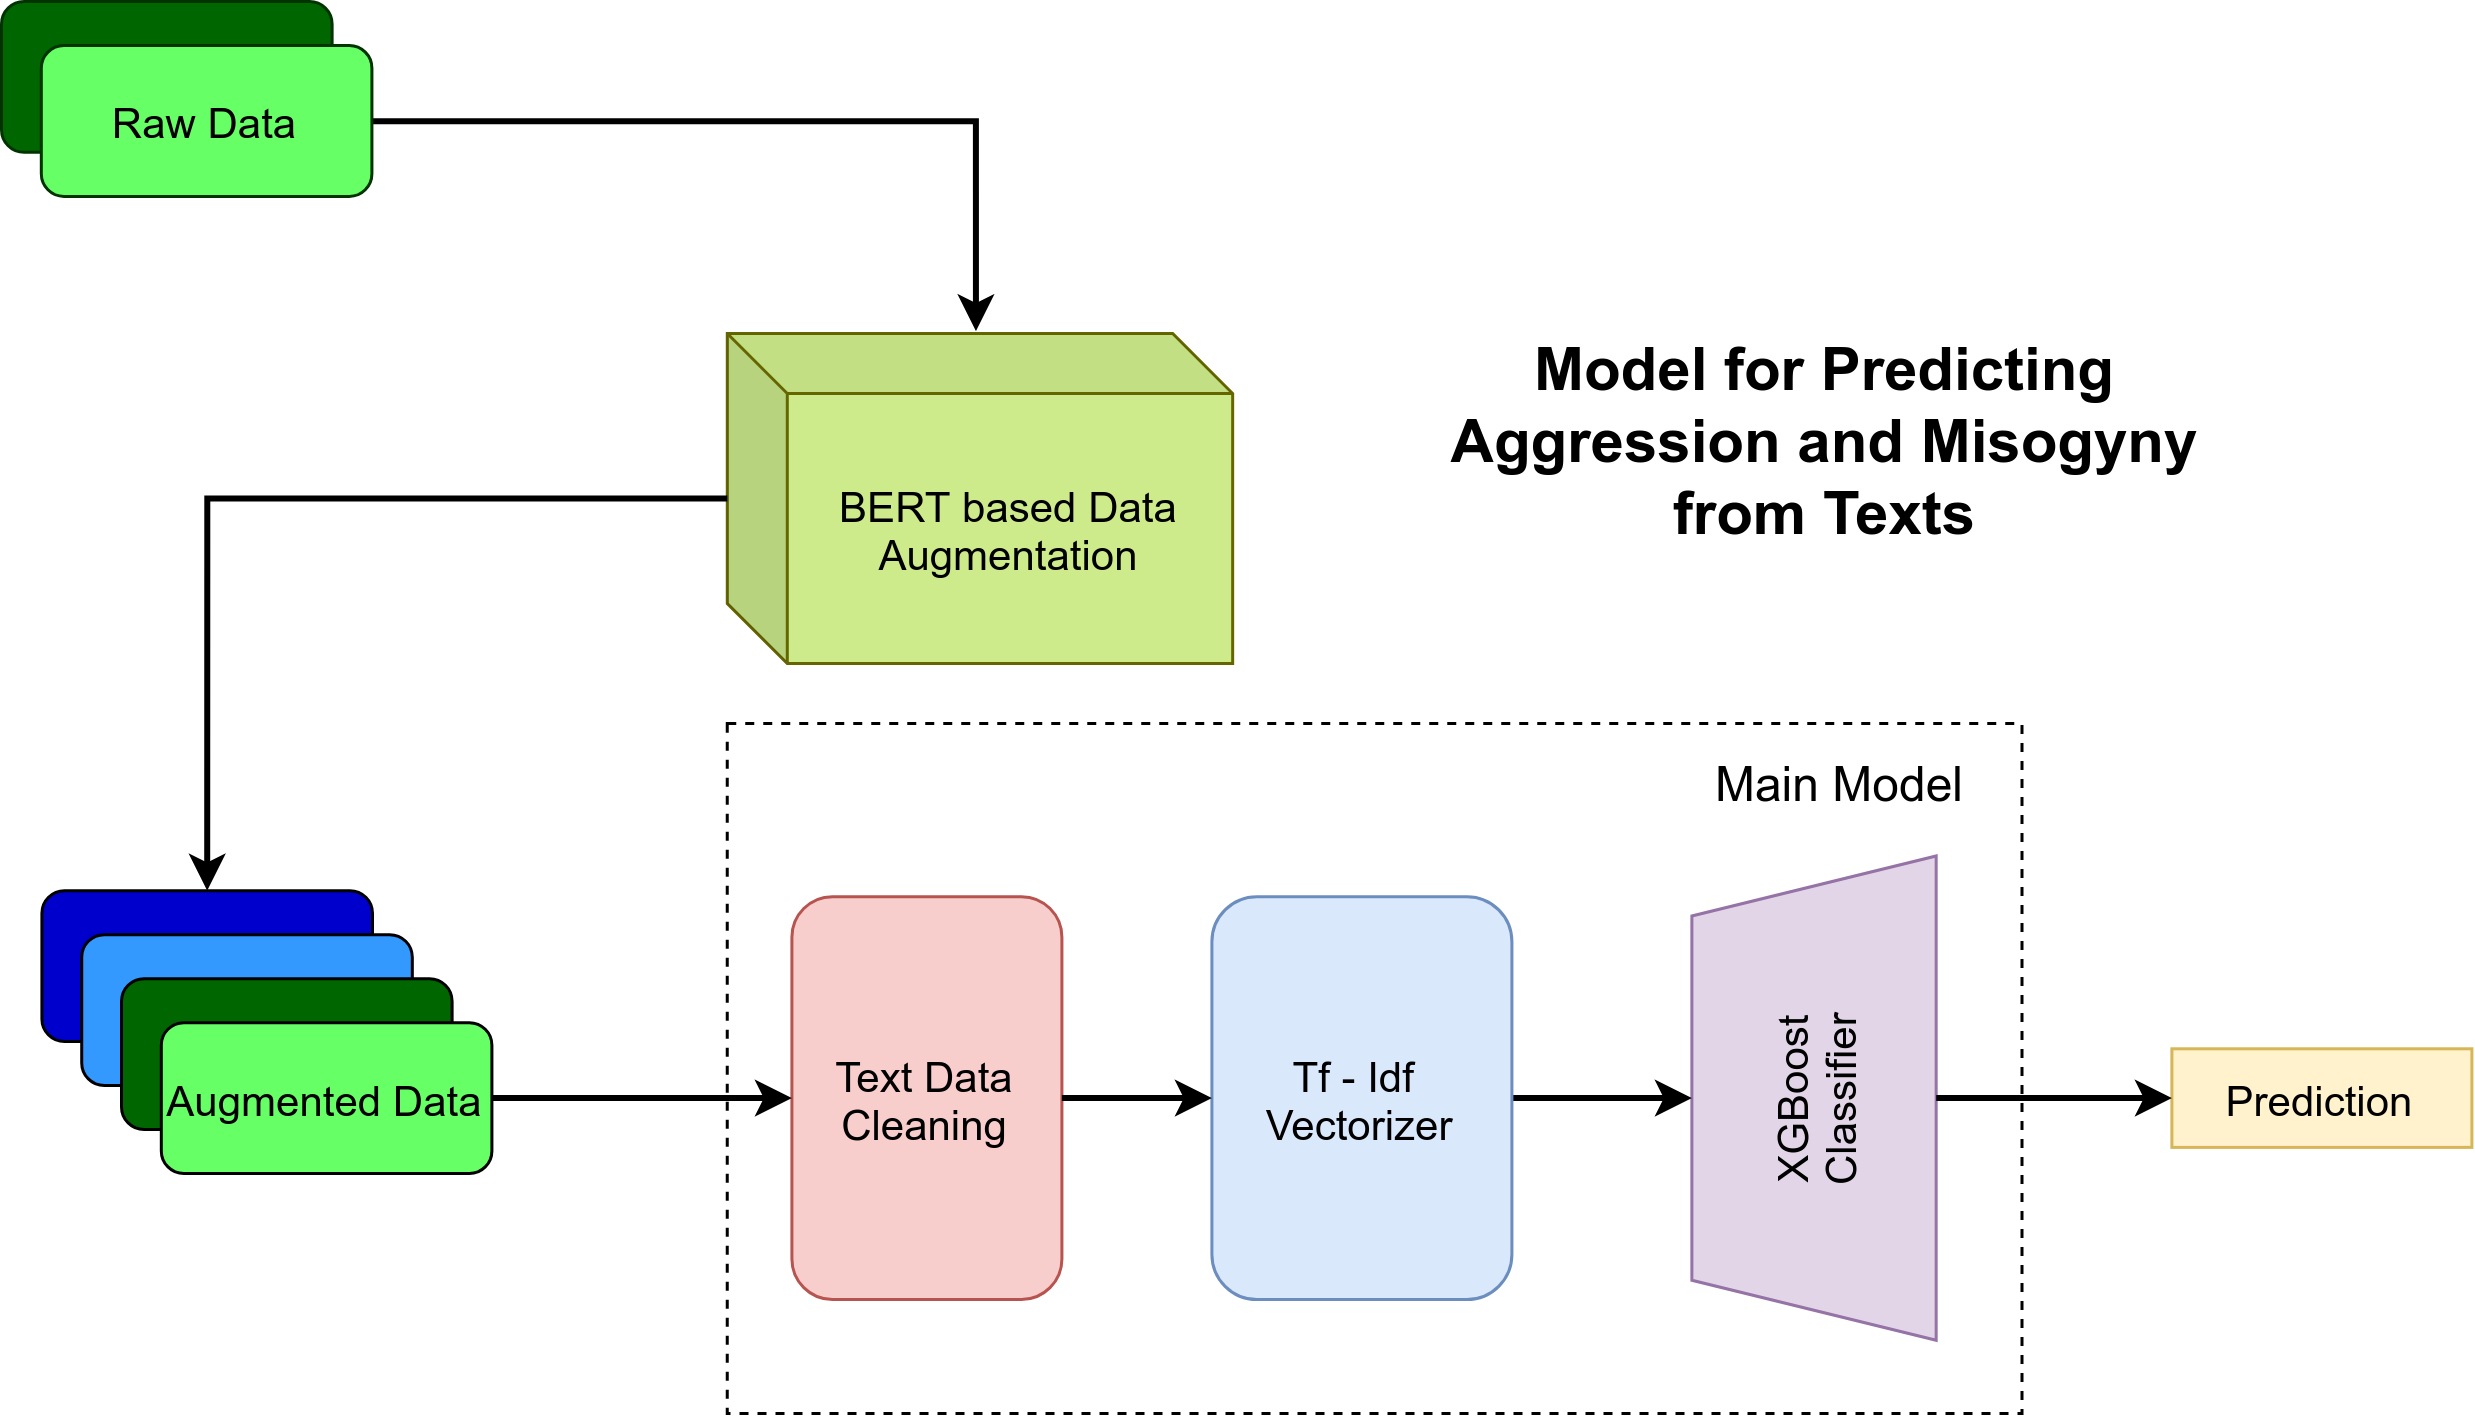
\includegraphics[scale=0.7]{assets/nn-1.png}
        \caption{Model Pipeline}
        \label{fig:pipeline}
    \end{center}
\end{figure*}
% -------MAIN IDEA-------------
\section{Model Pipeline}

\subsection{BERT based Text Data Augmentation}\label{subsec-bert-aug}
The data set had a skewed distribution, with the majority of the predictions belonging to one category. This imbalance can cause models to always predict the majority class. The model might give a very high score on the training data. However, it does not learn representations that can be useful for predictions. 

To counter this effect, the data was augmented. Data Augmentation generates additional data by generating slightly modified version of the original data. We employed a BERT based masked word prediction model for our purpose.

The process of augmentation is shown in Algorithm \eqref{algo:1}.

\begin{algorithm}[htbp]
\caption{BERT based Data Augmentation - Masked Word Prediction}
\label{algo:1}
\begin{algorithmic}[1]
    \STATE Select one text belonging to the minority class.
    
    \STATE Filter out the stop words from the text. Stop words are tokens like `is', `am' which do not contribute much to the overall sentiment of the sentence. Augmenting model with data having more of stop words will not be useful for our purpose. Hence we decide to remove them.
    
    \STATE Randomly select one token and replace it with a special \texttt{[MASK]} token. This token is understood by the BERT model. The model fills this token with the word that it deems to be most likely in that context.
    
    \STATE We take the top \texttt{k} predictions, where `\texttt{k}' is a hyper parameter. Typically, we want almost equal distribution for our classes so that the model may learn to classify all classes equally well. We choose k as per the data set.
    
    \STATE Repeat the above steps for other texts in the minority class to make the distribution even for all classes.
\end{algorithmic}
\end{algorithm}

The data set is augmented by using appropriate value of k and the results are stored. This computation essentially being a one time process, makes our overall pipeline faster. This process need not be repeated during inference, which makes our net model size smaller. 

\subsection{Text Data Cleaning}\label{subsec-clean}
To clean the texts, we use the following steps:\smallskip
\begin{itemize}
    \item \textbf{Remove Punctuation} -- Punctuation marks add unnecessary noise to the data. They are removed and replaced with space character.

    \item \textbf{Remove Stop Words} -- Stop Words do not contribute much meaning to our model. We use the default stop words of \texttt{nltk} package. However, removing some words like ``no'', ``not'', ``ain't'', ``won't'' changes the semantic nature of a sentence. Excluding these words, stopwords are replaced with the empty string. 
    
    \item \textbf{Stemming} -- Stemming converts words into their root form. This reduces vocabulary size and in turn the sparse word embedding dimensions. It also removes noise. \texttt{Porter Stemmer} from \texttt{nltk} package was used for this purpose.
\end{itemize}

\subsection{Tf--Idf Vectorization}\label{subsec-tf-idf}
Tf--Idf Vectorization is a scheme that converts a given text into a vector of numerical values. `Tf-Idf' stands for \emph{Term Frequency-Inverse Document Frequency}. It is a product of two terms $Tf(t)$ and $Idf(t)$, where:

\begin{equation*}
    Tf(t) = \frac{Frequency\ of\ term\ t\ in\ a\ sentence}{Total\ count\ of\ terms\ in\ that\ sentence} \bigskip
\end{equation*}


\begin{equation*}
    Idf(t) = log(\frac{Number\ of\ sentences\ in\ a\ document}{ Number\ of\ sentences\ which\ contains\ t})\bigskip
\end{equation*}

Classification task is made easier by using Tf--Idf, since taking the log of the inverse count of t term reduces the value of unimportant words occurring more frequently in the document.

Tf--Idf returns a sparse vector for each text. This helps reduce memory consumption and training times.

\subsection{XGBoost Text Classifier}\label{subsec-xgb}
XGBoost~\cite{chen2016xgboost} or Extreme Gradient Boosting is an extremely popular algorithm for classification. 

The reasons why this model is preferred:
\begin{itemize}
    \item \textbf{Sparsity Aware Computation} -- The previous step in our pipeline, \eqref{subsec-tf-idf} generates sparse vectors. It is undesirable that our model needs to convert them back into dense vectors, as that would lead to unnecessary computations. XGBoost supports computations on sparse data, which helps avoid unnecessary overheads and faster training.
    
    \item \textbf{Approximate Splitting Algorithm} -- For large data sets, fitting the entire data set in memory provides to be a challenge. Step \eqref{subsec-bert-aug} of our pipeline increases the amount of data in our data set by augmentation. XGBoost provides approximate methods for splitting the data which saves memory. Thus even after augmentation, the data can be fitted in memory.
    
    \item \textbf{Out of Core Computation} -- In case step \eqref{subsec-bert-aug} generates data which cannot be fitted into main memory, XGBoost chunks data into blocks and stores them on the disk. Thus even in the case of extremely large data, minimal changes need to be done to the model for training and inference.
    
    \item \textbf{Regularized Learning Objective} -- XGBoost provides regularized objective function, which controls model complexity and prevents over-fitting.
\end{itemize}
% ------------------------------TABLES --------------------------
% -----------------------Sub task A table------------------------
\begin{table}[!t]
\caption{Original Training Data Counts (English) for Sub Task A}
\label{table:sub-a-table}
\centering
    \begin{tabular}{|c|c|}
        \hline
        \textbf{Sub Task A Classes} & \textbf{Count per class} \\
        \hline
        NAG &  3375   \\
        CAG & 453    \\
        OAG & 435   \\
        \hline
    \end{tabular}
\end{table}

% ---------------------Sub task B table----------------------------
\begin{table}[!t]
\caption{Original Training Data Counts (English) for Sub Task B}
\label{table:sub-b-table}
\centering
    \begin{tabular}{|c|c|}
        \hline
        \textbf{Sub Task A Classes} & \textbf{Count per class} \\
        \hline
        NGEN  & 3954    \\
        GEN  & 309    \\
        \hline
    \end{tabular}
\end{table}
% -----------------------------------------------------------
% ---Table for All experiments performed----------------------
\begin{table*}[t]
\caption{Experiments on Various Classifiers and Weighted F1 Scores (Hyper-parameters not specified are Default Values)}
\label{table:all_experiments}
\centering
    \begin{tabularx}{\textwidth}
    {
        | >{\raggedright\raggedright}X 
        | >{\centering\arraybackslash}X 
        | >{\centering\arraybackslash}X |
    }
        \hline
        \textbf{Model} & \textbf{Sub Task A Score} & \textbf{Sub Task B Score} \\
        \hline
        Multi Layer Perceptron Classifier (50 iterations) & 0.533 & 0.720 \\
        Random Forest Classifier & 0.561 & 0.740 \\
        LinearSVC & 0.620 & 0.773 \\
        XGBoost Classifier & 0.729 & 0.852 \\
        XGBoost Classifier ($\gamma=0.2$) & 0.729 & 0.850 \\
        \textbf{Final Model -- XGBoost Classifier ($\gamma=0.1$)} & \textbf{0.735} & \textbf{0.852}\\
        \hline
    \end{tabularx}
    
\end{table*}
% -----------------------------------------------------------------
% -------------Results of the Table--------------------------------
\begin{table*}[t]
\caption{Results obtained (Weighted F1 Score)}
\label{table-results}
\centering
    \begin{tabularx}{\textwidth}
    {
        | >{\raggedright\arraybackslash}X 
        | >{\centering\arraybackslash}X 
        | >{\centering\arraybackslash}X |
    }
        \hline
        \textbf{Team Name} & \textbf{Sub Task A Score} & \textbf{Sub Task B Score} \\
        \hline
        Julian\cite{risch2020offensive} & 0.802 & 0.851 \\
        abaruah\cite{baruah-etal-2020-aggression} & 0.728 & 0.870 \\
        sdhanshu\cite{Niloofar-etal-TRAC2020-AggressionDetection-BERT-MultiTask} & 0.759 & 0.857 \\
        \textbf{Our Team Results} & \textbf{0.735} & \textbf{0.852}\\
        \hline
    \end{tabularx}
\end{table*}
% ---------------------------------------------------------------------


% ----------EXPERIMENTS AND RESULTS-----------------
\section{Training and Results}\label{sec-exp-res}
\subsection{Data set Description}
The data set we used for our model was obtained from \cite{trac2-dataset}. The English data set was used for our purpose. 

The data set consisted of texts scraped from YouTube comment section
\cite{TRAC:2020}. Two target features were provided by the organisers, `Sub Task A' and `Sub Task B'.

Sub Task A required us to use detect the level of aggression in a text. One of 3 given classes needed to be predicted:
\begin{itemize}
    \item \textbf{Non Aggressive (NAG)} - Posts do not contain any aggressive content
    \item \textbf{Covertly Aggressive (CAG)} - Posts contain some aggressive content disguised as other forms of speech, e.g, sarcasm
    \item \textbf{Overly Aggressive (OAG)} - Posts contain direct aggressive content
\end{itemize}

Sub Task B consisted of misogynistic language identification. The classes were:
\begin{itemize}
    \item \textbf{Non Misogynistic (NGEN)} - Posts do not contain any misogynistic content
    \item \textbf{Misogynistic (GEN)} - Posts do not contain any misogynistic content
\end{itemize}

As shown in Table \eqref{table:sub-a-table} and Table \eqref{table:sub-b-table}, there was a huge imbalance in terms of class distribution. This was fixed by using BERT based augmentation and then prediction was done using the pipeline as described in \eqref{subsec-clean} -- \eqref{subsec-xgb}.

\subsection{Experimental Setup}
The entire pipeline was trained on Google Colab environment.

A number of experiments were performed using \texttt{scikit-learn} \cite{scikit-learn} which have been shown in Table\eqref{table:all_experiments}. 
The hyperparameters which have not been mentioned in Table\eqref{table:all_experiments} were all set to their default value as provided by the library.

Hyper-parameter \texttt{k} (Algorithm \eqref{algo:1}) was set to 2 for our model to augment each data point 2 times. 
This entire process was repeated 2 times to even out the distribution.

The BERT masked word prediction augmentation model was moved to the GPU (available in Colab) but not fine tuned. Number of self attention heads was set to 12. The hidden layer size was set to 768. All other hyper parameters were set as described in \cite{DBLP:journals/corr/abs-1810-04805}. It took about 10 minutes for finishing the entire data augmentation process on a Nvidia Tesla K80 GPU.

Next, the Tf-Idf + XgBoost pipeline was trained on an Intel Xeon CPU. The \texttt{gamma} hyperparameter of XGBoost model was set to 0.1 for added regularization. All other hyper parameters were kept to their default values. The entire process of cleaning, training, validation and predicting on test data took about 2 minutes to complete.

The metric used for evaluation was weighted F1 score.

\subsection{Results and Comparison}
The results obtained are elucidated in Table \eqref{table-results}.

The highest scores achieved in this task by \cite{risch2020offensive} used bagging of multiple BERT models for prediction. Their entire pipeline required 7 hours to train on a Nvidia 1080 Ti GPU. \cite{Niloofar-etal-TRAC2020-AggressionDetection-BERT-MultiTask} took about 6 hours for training the entire model with a Nvidia Tesla P40 GPU.

Other top performing models \cite{baruah-etal-2020-aggression} all used Transformer based models, which demands heavy computational resources.

Our model achieves nearly the state of the art for this task.
However, the entire pipeline requires only a small fraction of the computational resources and time that the top models need. To train the model, the total time required is  about 30 minutes, which is drastically lower compared to top performing models.

The storage size occupied by our model is also lower. Our models occupy about few MB's (\texttt{.pkl} files), whereas other models take hundreds of MB's for storing their BERT based pipelines.
% ----------ANALYSIS-----------------------
\section{Performance Analysis}
% ----------Binary Classification Table----------------
\begin{table}[t]
\caption{Confusion Matrix for Binary Classification}
\label{table:tab-5}
\centering
    \begin{tabular}{|c|c|c|}
        \hline
        \textbf{Predicted(row) / True(column)} & \textbf{Positive} & \textbf{Negative}\\
        \hline
        Positive & TP & FP   \\
        Negative & FN & TN    \\
        \hline
    \end{tabular}
\end{table}
%---------------------------------------------------
In this section, the model is analysed for performance and error susceptibility. For this task, a confusion matrix is developed for each task to determine the extent of false negatives and false positives predicted by the model. 

A confusion matrix, also known as an error matrix, is a specific table layout that allows visualization of the performance of an algorithm. Each row of the matrix represents the instances in an actual parameter while each column represents the instances in a predicted parameter, generally. The name stems from the fact that it makes it easy to see whether the system is confusing two classes.

Table \eqref{table:tab-5} shows a confusion matrix for binary classification. In the table, TP denotes True Positive (predicted as true and is actually true), FP denotes False Positive (predicted
as true but is actually false), FN denotes False Negative (predicted as false but is actually true) and TN denotes True Negative (predicted as false and is actually false).

For Task-A, a 3 $*$ 3 matrix is constructed and obtained, since it has three categories - NAG, CAG, OAG. Figure \eqref{fig:heatmapA} shows the confusion matrix for Task-A, namely Aggression Detection.

For Task-B, a 2 $*$ 2 matrix is constructed and obtained, since it has two categories - NGEN, GEN. Figure \eqref{fig:heatmapB} shows the confusion matrix for Task-B, namely Misogyny Detection.

\begin{figure}[t!]
    \centering
    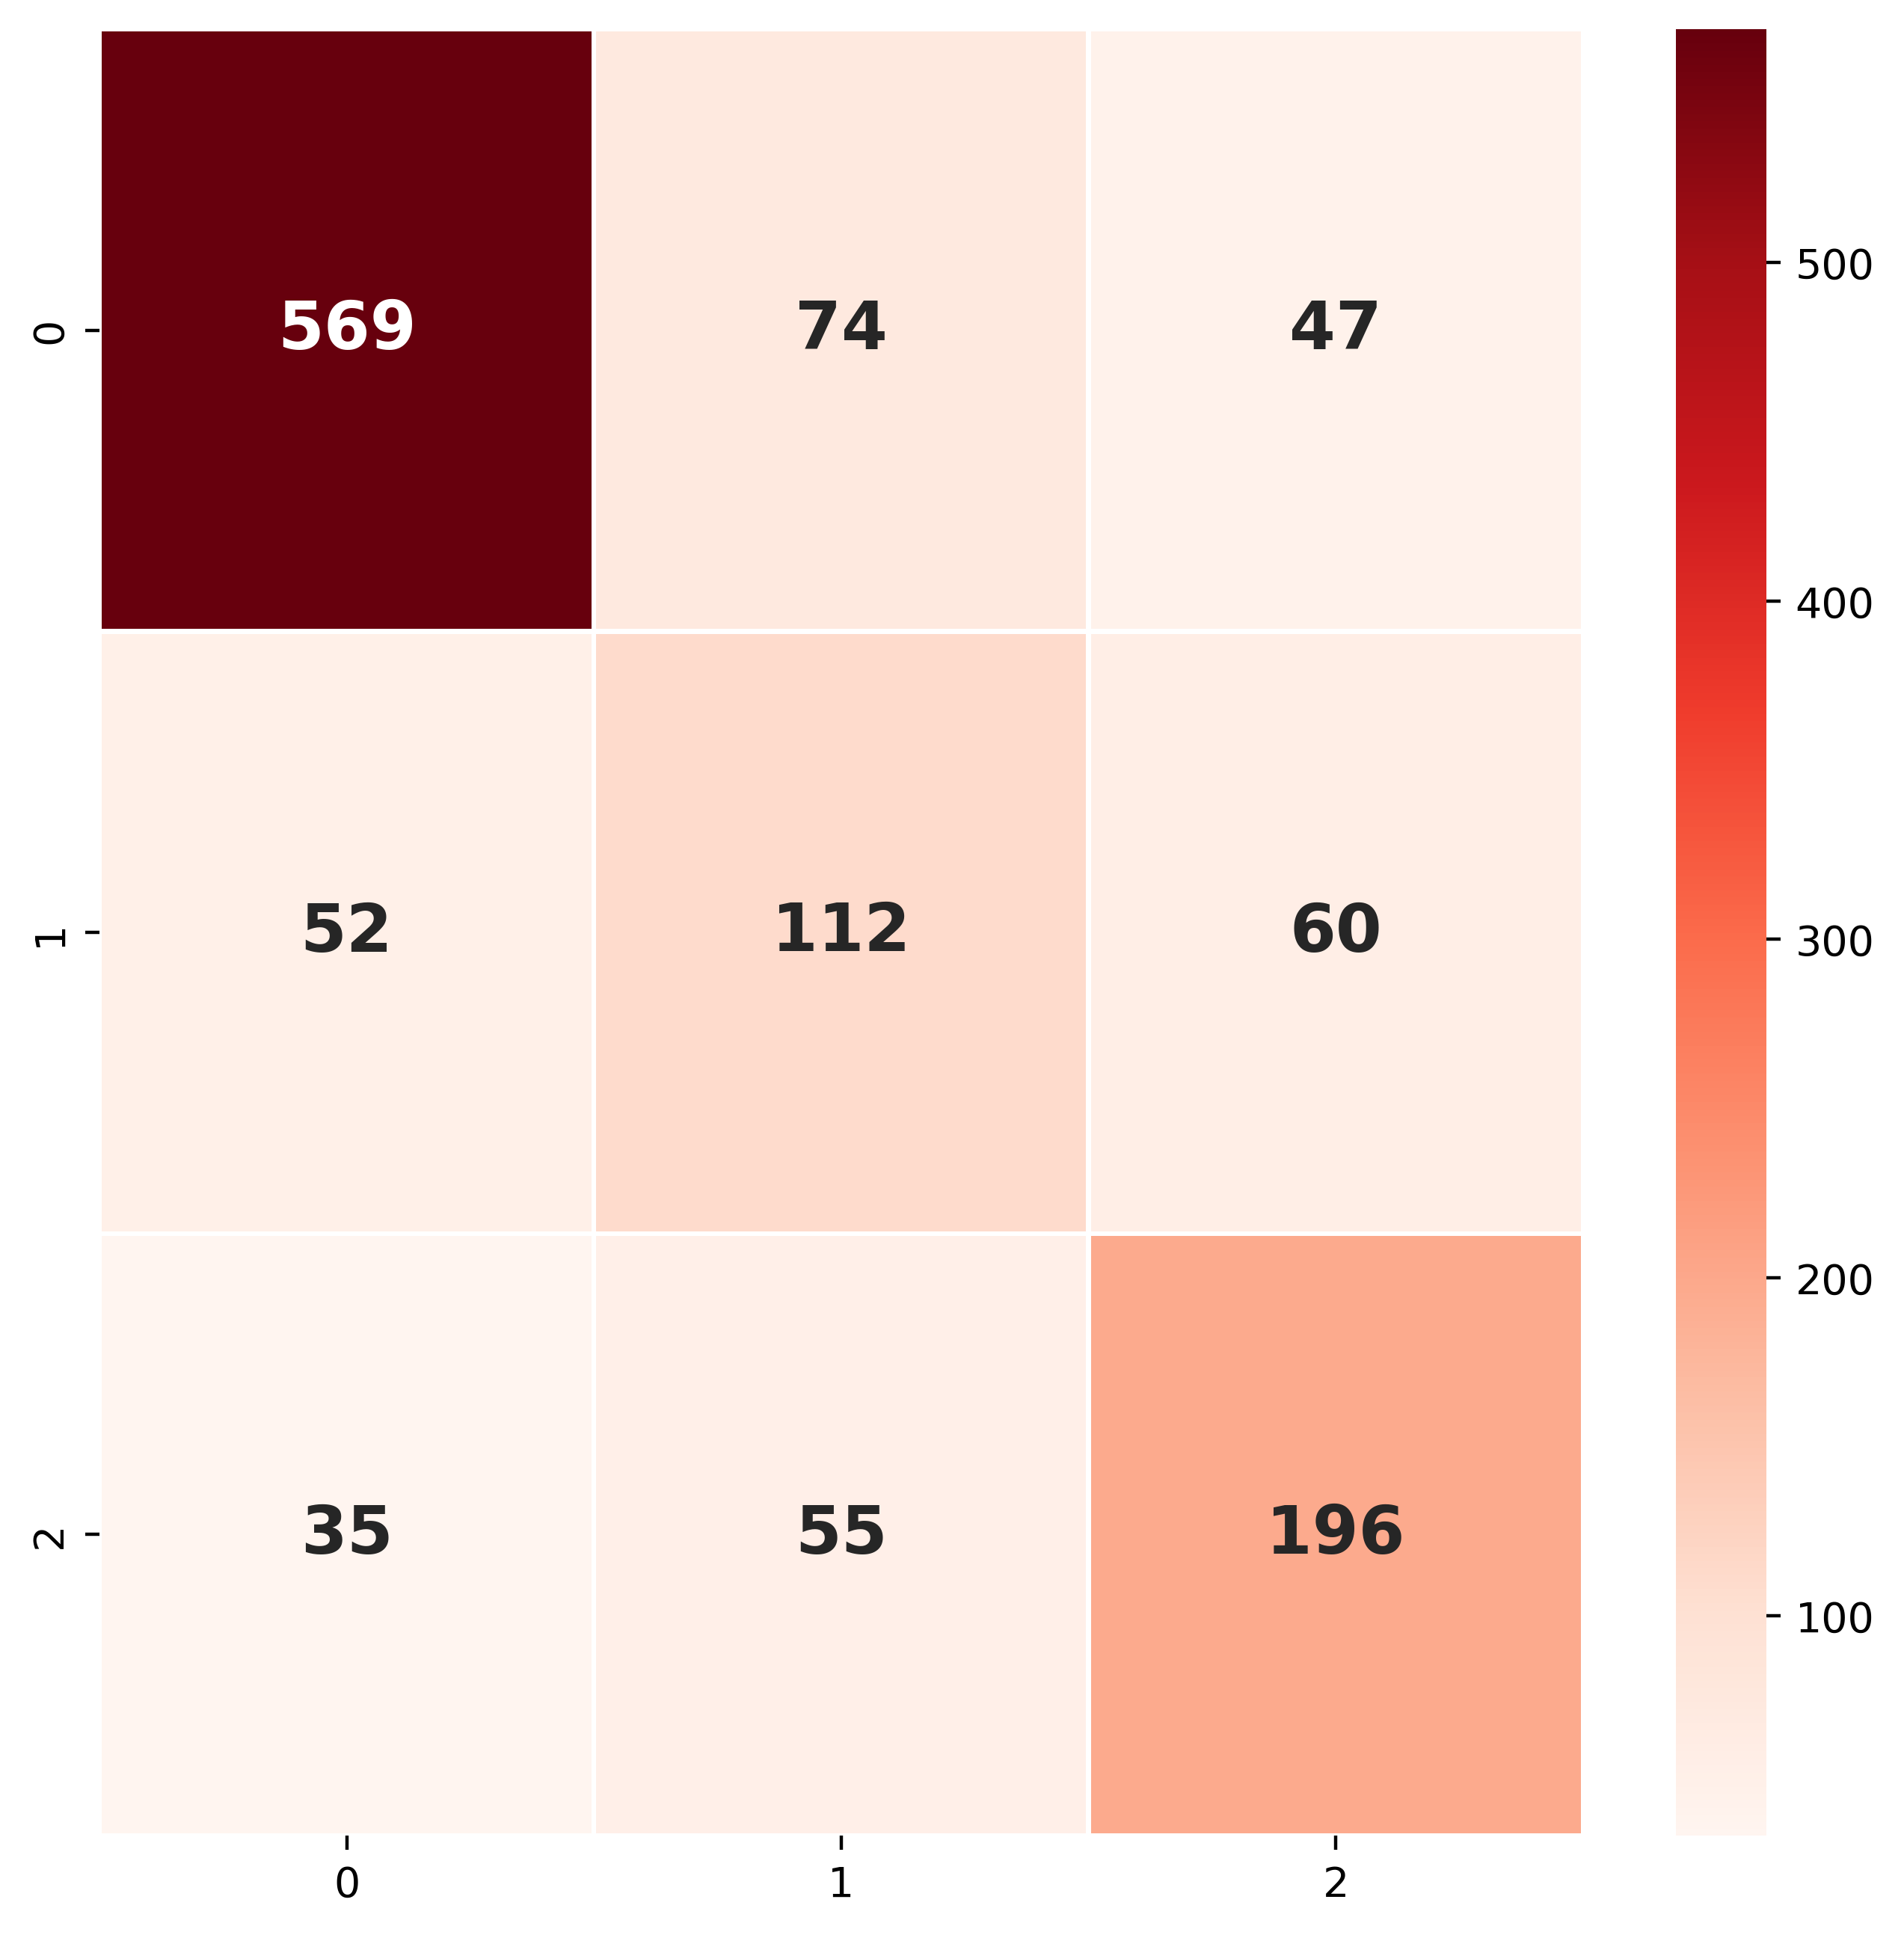
\includegraphics[scale=0.5]{assets/heatmap_task_A.png}
    \caption{Confusion Matrix of Task A. (0 - NAG, 1 - CAG, 2 - OAG)}
    \label{fig:heatmapA}
\end{figure}

\begin{figure}[t!]
    \centering
    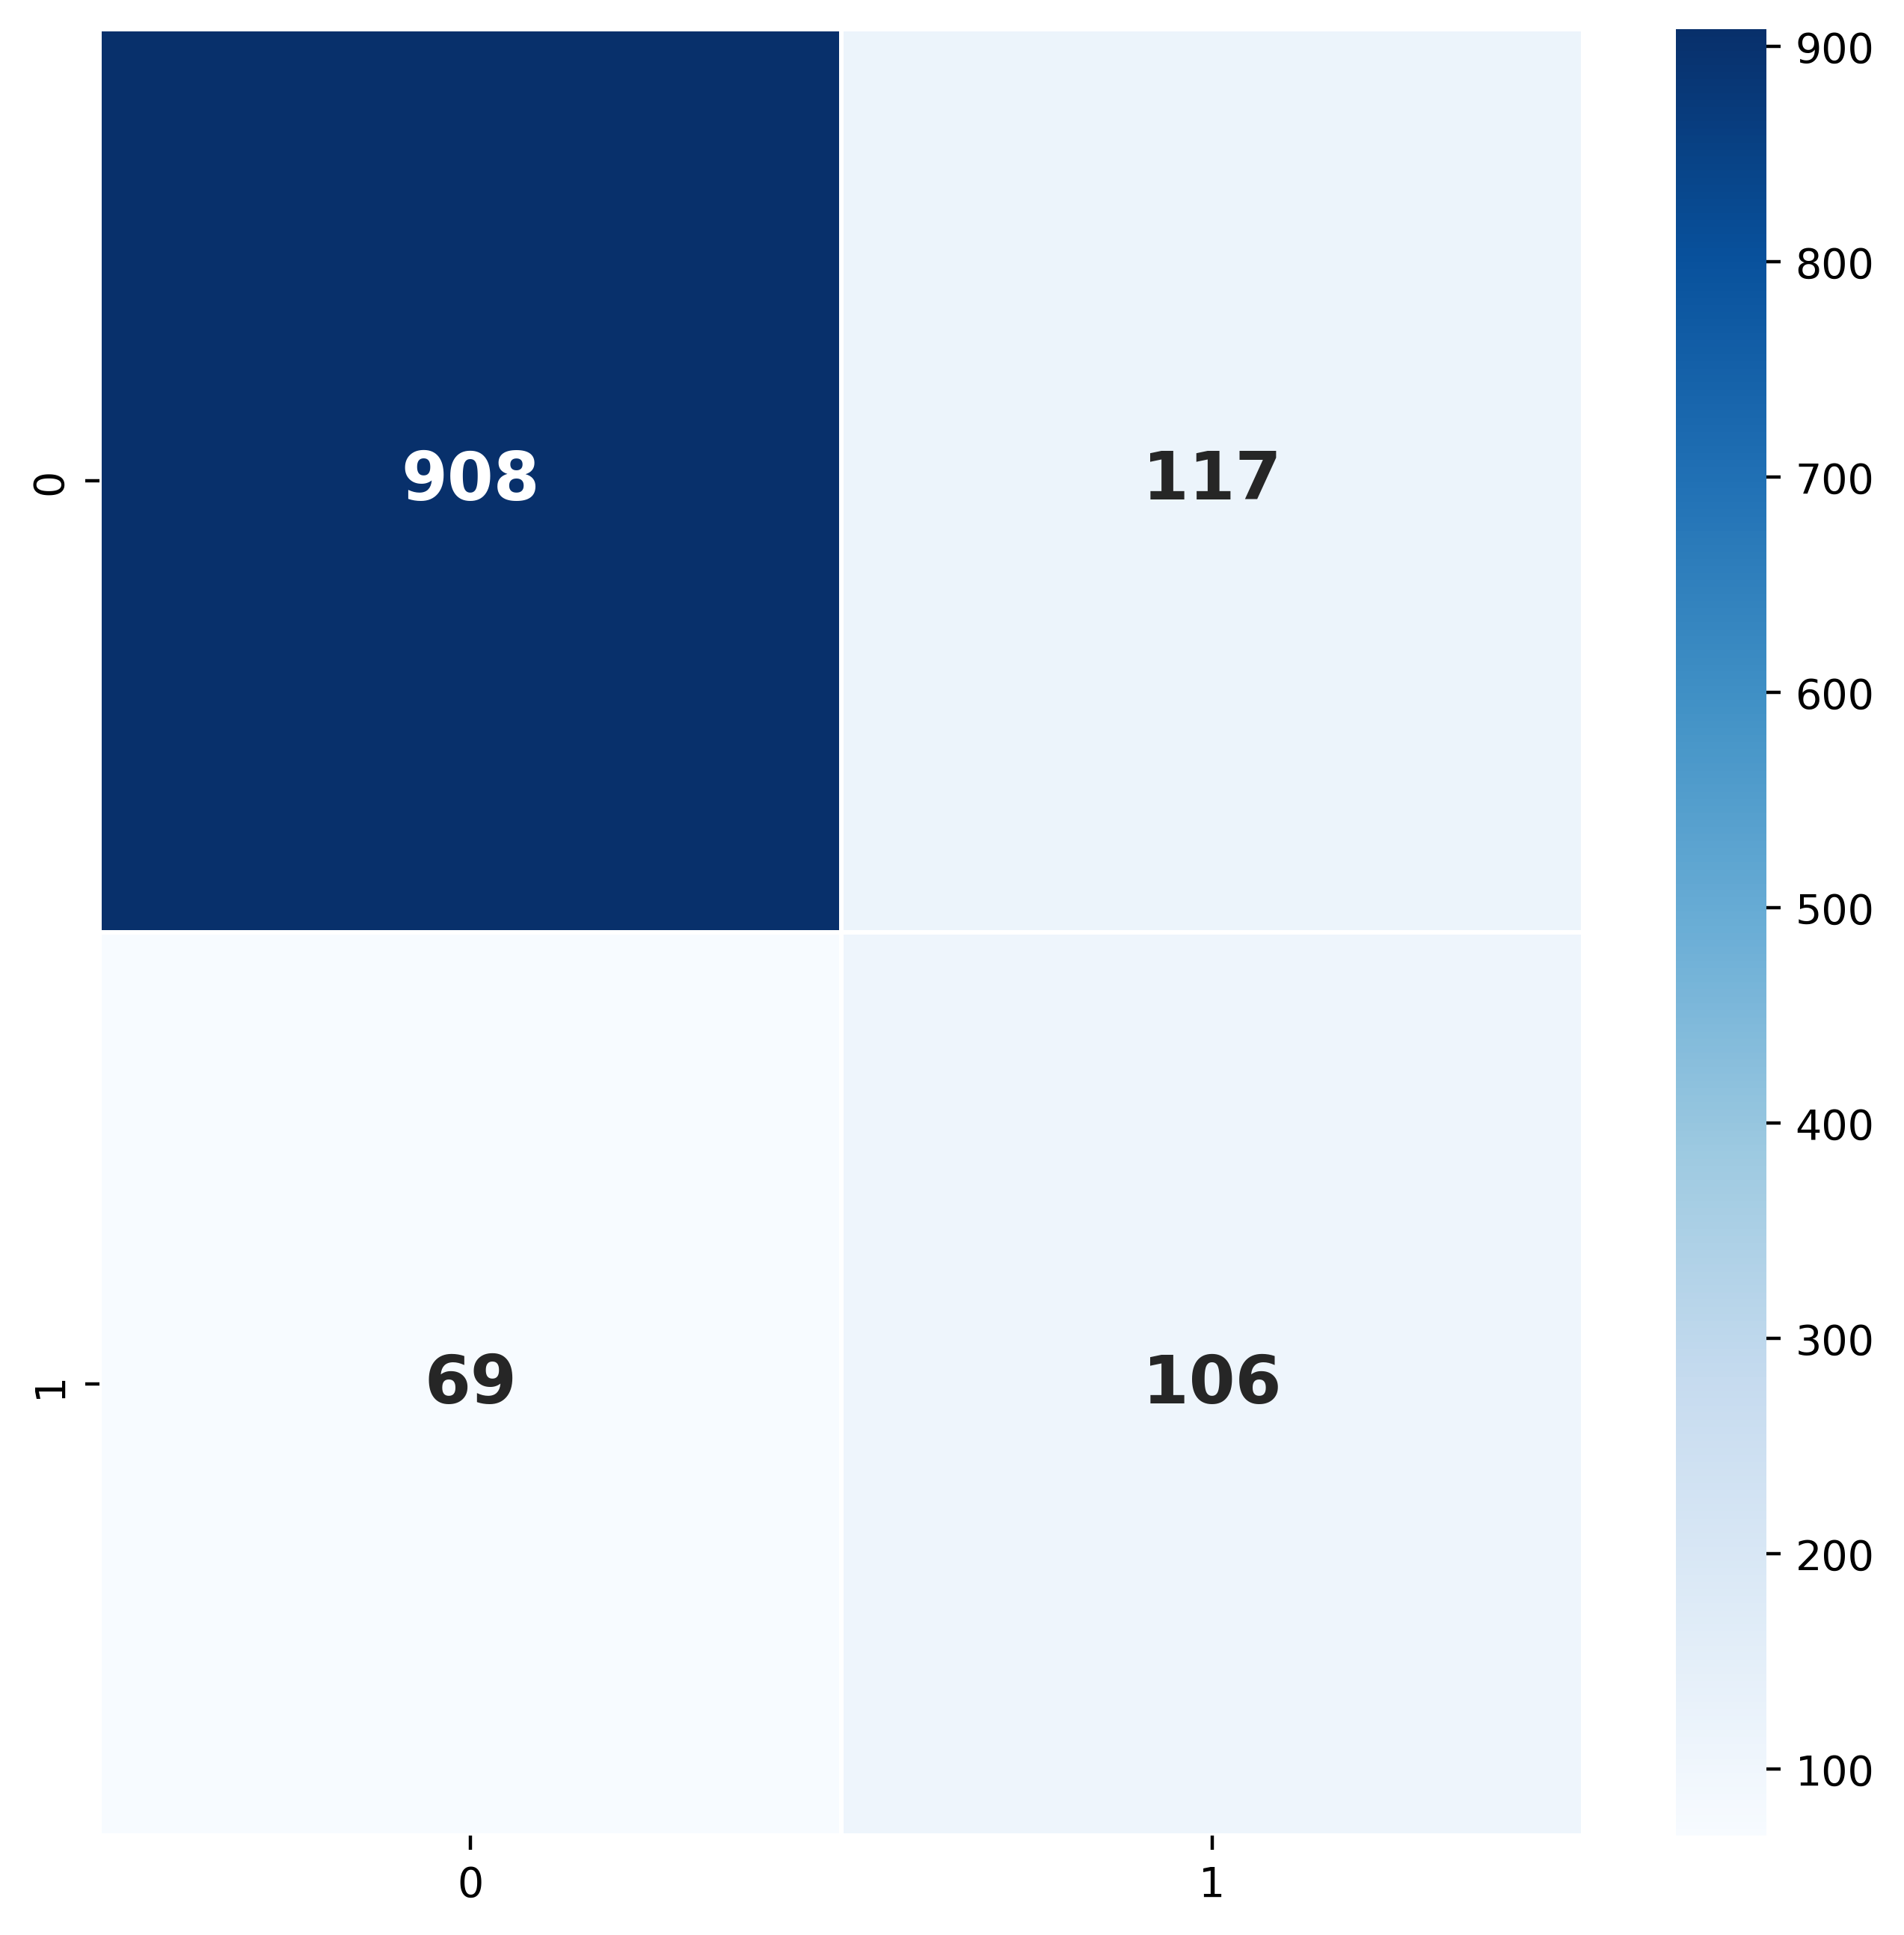
\includegraphics[scale=0.5]{assets/heatmap_task_B.png}
    \caption{Confusion Matrix of Task B (0 - NGEN, 1 - GEN)}
    \label{fig:heatmapB}
\end{figure}

Lastly, the classification report for each task is obtained and can be concluded that the model has performed satisfactorily, based on model accuracy and weighted f1-scores. Tables \eqref{table:tab-6} and \eqref{table:tab-7} show the given values.

We see that our model detects non aggressive and overtly aggressive categories fairly well. However, the performance on detecting covertly aggressive data is relatively lower. Our model shows some problem in detecting aggression in covert forms such as in sarcasm. For the second case, our model performs shows some degradation in performance when detecting misogyny. 

% Classification Table A
\begin{table}[t]
\caption{Classification Report of Task A}
\label{table:tab-6}
\centering
    \begin{tabular}{|c|c|c|c|c|}
        \hline
        \textbf{ } & \textbf{precision} & \textbf{recall} & \textbf{f1-score}  & \textbf{support}\\
        \hline
        0 (NAG) & 0.87 & 0.82 & 0.85 & 690   \\
        1 (CAG) & 0.46 & 0.50 & 0.48 & 224   \\
        2 (OAG) & 0.65 & 0.69 & 0.67 & 286   \\
        accuracy & - & - & 0.73 & 1200 \\
   macro avg & 0.66 & 0.67 & 0.66 & 1200 \\ 
weighted avg & 0.74 & 0.73 & 0.73 & 1200 \\
        \hline
    \end{tabular}
\end{table}

% Classification Table B
\begin{table}[t]
\caption{Classification Report of Task B}
\label{table:tab-7}
\centering
    \begin{tabular}{|c|c|c|c|c|}
        \hline
        \textbf{ } & \textbf{precision} & \textbf{recall} & \textbf{f1-score}  & \textbf{support}\\
        \hline
        0 (NGEN) & 0.93 & 0.89 & 0.91 & 1025   \\
        1 (GEN) & 0.48 & 0.61 & 0.53 & 175   \\
        accuracy & - & - & 0.84 & 1200 \\
   macro avg & 0.70 & 0.75 & 0.72 & 1200 \\ 
weighted avg & 0.86 & 0.84 & 0.85 & 1200 \\
        \hline
    \end{tabular}
\end{table}

% ----------CONCLUSION------------------------------
\section{Conclusion}
In this work, a fast and efficient pipeline to detect aggression and misogyny from social media texts was developed. The model was trained and the obtained score was recorded and compared to other models. Error analysis was performed to understand the results. 
% ----------ACKNOWLEDGEMENTS------------------------
% \section*{Acknowledgment}


% --------BIBLIOGRAPHY------------------------------
% cite as \cite{bib-key-1}, \cite{bib-key-2} etc
\bibliographystyle{IEEEtran}
\bibliography{./references/references}{}
% ----------END-----------------------
\end{document}